%-----------------------------------------------------------------------------------------
\clearpage
\section{Implementation}
%-----------------------------------------------------------------------------------------
In this section we describe how the project is implemented in detail. The subsystems executed are data reading, visualisation rendering and the user options. Screen captures of the GUI are added to illustrate further information.

\subsection{Data Processing}

The main concept of data processing is to read text data from .txt files, calculate values need, and store them into Java Arraylist. At this stage, the greatest challenge is to keep the data being accessible and can be changed, as  the new data may be written over the old due to events in other class. Hence, after the original data is read and stored, it is retrieved and modified through  mutator methods \cite{Laramee2013}. In addtion to the flexibility, another difficulty at this stage is generating values for each term and store them appropriately. As discussed in the Project Features section, the aim of the software we designed is to present information about terms and provide an concordance view for each version. In this project, we calculate and sort frequencies of terms; compute colour values; computed locations of strings; instantiate Rectangle objects to represent data; create arrays to store translations.

Java.io, which enables for system input and output through data streams, is used in this project. It serves as a data buffer and reader in this project. The FileReader class, which extends the InputStreamReader class, can be used to read character files which by default are assumed to be an appropriate size. Since the volume of data in each document is not large, we instantiate a FileReader (object) to access each text file. The other data reading class adopted is the BufferedReader class. It is used to read text data from a character-input stream, and buffer the data to provide efficient reading of strings, arrays and lines \cite{Gosling2014}. Java.util is another package imported in the DataReader class. To store and access data, the ArrayList, Hashtable, and Map classes from this package are used. In addition, classes such as JsonObject, JsonReader, and JsonArray in Javax.json package are used to read data from a Json file.

The main class that is responsible for reading the original data file is the DataReader class. This class analyses .txt files and generates a list of Version objects to parse all information needed in the software. Each Version object stores information of the concordance. For a more detailed description of the Version class and Item class, please see the Design section.

\subsection{Generating Concordances}

Concordances are the most basic visualisation in this project. They are designed to display the information of terms, and to help in comparing the terms between different translation versions.As shown in the Figure \ref{fig:condorVis}, the concordance visualisation involves several parts:
\begin{figure}[H]
	\centering	
	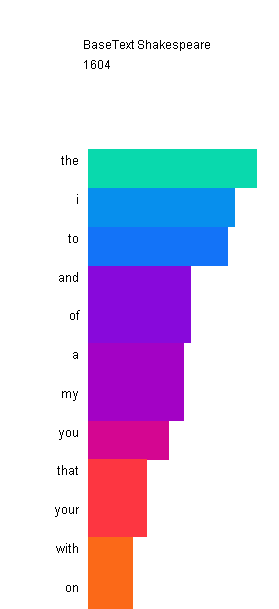
\includegraphics[width=9cm, height=15cm]{Figs/condordanceVis}\\[1ex]
	\caption{The Screenshot of one concordance in the visualisation}
	\label{fig:condorVis}
\end{figure} 

\begin{itemize}
	\item \textbf{String} is drawn to display the term, frequency, version author, publication year; 
	\item \textbf{Rectangle} is used to present the frequency. As the values are sorted in data processing phase, the width of rectangles are set according to these sorted values.
	\item \textbf{Colour} is used to present differences on frequency. The colour of the word is calculated used its frequency number. 
\end{itemize}

The process in generating the concordance visualisation goes through the following steps:
\begin{itemize}
	\item \textbf{} Obtain the string of each term from text source. This step is done in the DataReader class. Detailed illustration seeing Data Reading implementation section.
	\item \textbf{} Calculate the number of times, namely term frequency, each term occurred in the text (See Data Reading implementation section).  	
	\item \textbf{} Calculate the rectangle width for each term using the frequency of term. The equation of the rectangle width calculating is show in Equation \eqref{rectWidth}:
	
	\begin{multline}\label{rectWidth}
	rectWidth=wordFrequency*unit*scaleValue
	\end{multline}
	
	Where unit is the width of each segment since the rectangle is composed of a number of segments. WordFrequency is the value deciding how many segments compose the rectangle, while scaleValue is the percentage value used to scale the rectangle, range from 10\% to 200\%.
	
	\item \textbf{}Calculate the location of the string and rectangle.The location, or point, is the start drawing point for the string and rectangle. It combined with two point value: point.X, and point.Y. The Equation \eqref{PointX}, \eqref{PointY} illustrate how we calculate these points in the software:
	
	\begin{multline}\label{PointX}
	point.x=versionNumber*versionDistance*scaleValue
	\end{multline}
	
	\begin{multline}\label{PointY}
	point.y= lineNumber*lineDistance*scaleValue
	\end{multline}
	
	Where versionNumber represents order number of the version. versionDistance performs the  distance between two neighbour versions. In addition, a scale value need to be multiplied so that the location of string and rectangle changes according to user preference.
	Similarly, the lineNumber is order number of the term while lineDistance represents the distance between two terms. 
	
	\item \textbf{}Calculate the value of colour. According to \cite{Jbum}, we use the equation as shown in Equation \eqref{Red}: 	



	\begin{multline}\label{Red}
	color = Math.sin(colorFrequency*wordFrequency + phase) *\\ amplitude + center
	\end{multline}


	Where colorFrequency is a constant that controls how fast the wave oscillates. The wordFrequency is  variable used to display different colour according to word frequency. The phase is applied to change the alignment of the green or blue sine waves. The amplitude controls how high (or low) the wave goes. The center controls the center position of the wave.
	
	\item \textbf{}Paint the strings, blocks, and colours by invoking drawing methods in Graphic class. 
	
\end{itemize}

\subsection{Parallel View of Concordances}

Following the generation of the Concordance visualisation, a parallel view of all concordances is created, as shown in Figure \ref{fig:parallelConcor}. During this stage, lines are drawn to highlight identical terms. The comparison stage is done in the ConcordancePanel class. 

\begin{figure}[H]
	\centering	
	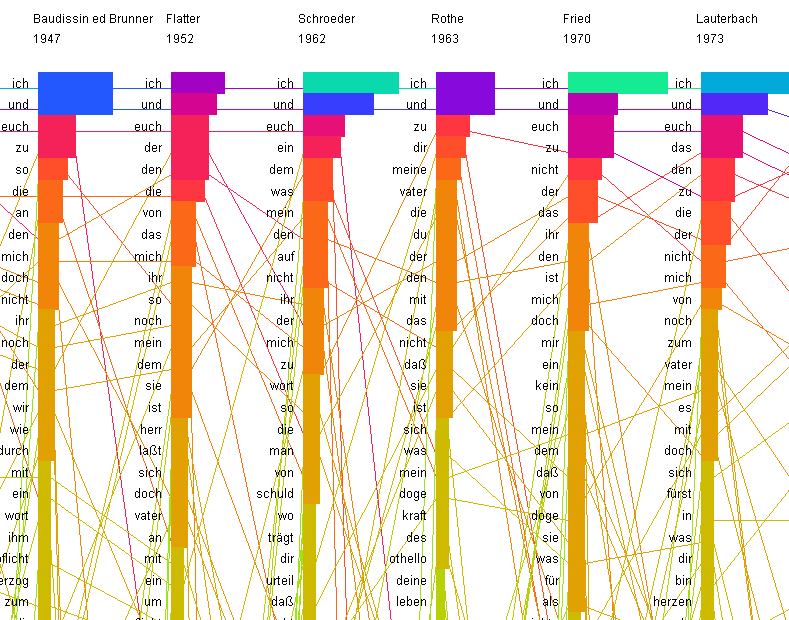
\includegraphics[scale=0.6]{Figs/Parallel-Vis}\\[1ex]
	\caption{Parallel view of concordances.}
	\label{fig:parallelConcor}
\end{figure} 


However, after this parallel visualisation is generated, an obvious problem appears, there is not enough space for all 16 concordances to be shown simultaneously. Therefore the solution is either to scale the panel, or to select several versions for showing at one time. We have included both solutions, which are detailed in the following section. 

\subsection{Zooming}

Zooming in and out is a basic feature in the software which is designed to provide two zooming options: one is for scaling the content of the visualisation, the other is for scaling the frame. In addition to these two scaling options, there are also scroll bars used to scroll the visualisation panel.

To implement these features, several steps as followed are gone through:
\begin{itemize}
	\item \textbf{} Generate the JSlider objects. This is carried out in the TranslationVisualization class. Figure \ref{fig:jSliders} displays the JSlider applied in the software.
	\begin{figure}[H]
		\centering	
		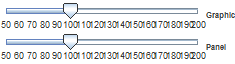
\includegraphics[scale=1]{Figs/JSliders}\\[1ex]
		\caption{The screenshot of the JSliders.}
		\label{fig:jSliders}
	\end{figure} 	
	\item \textbf{} Obtain scale values from JSlider object and pass them to DataReader class.
	\item \textbf{} Recalculate the data by invoking the calculating methods such as calculatePoint() and setRectWidth().
	\item \textbf{} Update the List<Version> object.
	\item \textbf{} Repaint graphics.
\end{itemize} 
 
During this process, the most difficult part is to recalculate all values of graphics: points, widths and heights for rectangles, and the distances between versions. To overcome this dilemma, two solutions are attempted:
At the first phase, scale() method in Graphics2D class is invoked. By applying this method, computer will calculate and repaint all the graphics using scale parameters passed in. However, when the project prompting to the Term Selecting phase (See Interactive Selection of Terms section below), a problem of obtaining mouse clicking location appears. Hence, the second phase of scaling visualisation comes out.  

At the second phase, scale values attained from JSlider objects are passed to DataReader class and applied in relevant formulas to calculate variables such as points, widths and heights of rectangles. See Equation \eqref{rectWidth}, \eqref{PointX}, and \eqref{PointY}. As shown in \ref{fig:jSliders}, 100 is set as the initial value for the slider, so that the visualisation shown when the visualisation generated at the first time is scaled as 100\%. 
\subsection{Text Label Toggling}

As the scale values become smaller, the strings begin to overlap. This inspires a new feature; toggling labels in the visualisation, enabling users to focus only on the rectangles and colours. Next, an event listener is registered to the JButton. When the button is clicked, its label value is replaced by “Text Off”. Consequently, with the default state ‘true’ is toggled ‘false’, then passed to the ConcordancePanel class. In the third step, a boolean value preset when drawing strings of terms will be assigned the same truth value as the boolean passed in. If it is true”, then draw the strings, else if it is ”false” then do not the drawString() method. Finally, we repaint the graphic. Figure \ref{fig:textOnOff} is a screenshot of concordance view with labels toggled off.

\begin{figure}[H]
	\centering	
	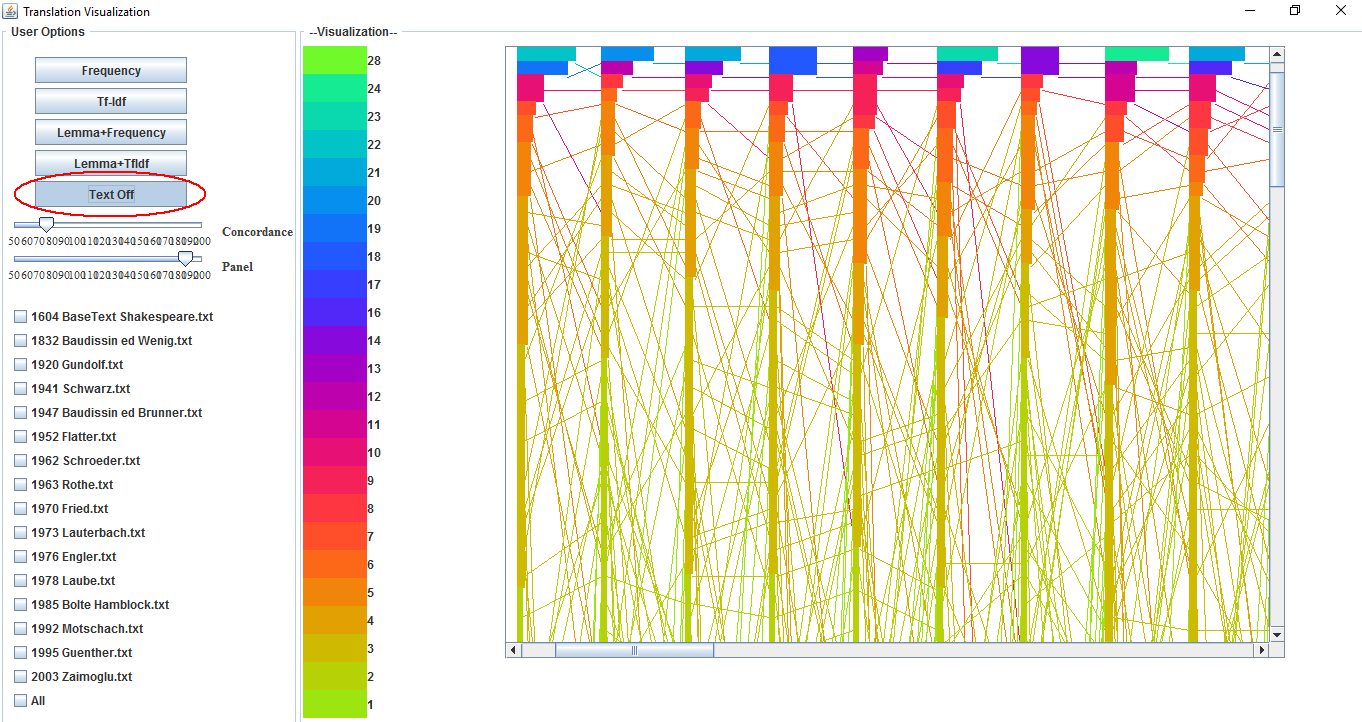
\includegraphics[width=\textwidth]{Figs/Text-On-Off}\\[1ex]
	\caption{Results of toggling off text.}
	\label{fig:textOnOff}\textsl{}
\end{figure} 

\subsection{Adding, Subtracting, Selecting Items}

To render the user option feature for selecting several concordances displaying on the panel, a new class called VersionChosenPanel is created. By interacting with this feature, not only can the user select which concordance to display in the visualisation, but also the order in which they are displayed. Figure
\ref{fig:versionChoosPanel} shows the menu where users can select which versions to display. 
\begin{figure}[H]
	\centering	
	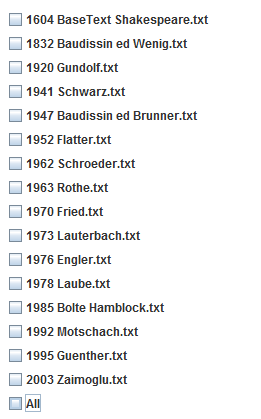
\includegraphics[scale=0.5]{Figs/VersionChoosePanel}\\[1ex]
	\caption{Version selection menu.}
	\label{fig:versionChoosPanel}
\end{figure} 

To implement the version selection feature we did the following steps:
\begin{itemize}
	\item \textbf{} Rendering a list of JCheckBox objects to display the author name as the index. 
	\item \textbf{} An event listener for each JCheckBox object, so that the action of selection can be generated as an object of class Object.
	\item \textbf{} Toggle the selecting status of the index. 
	\item \textbf{} Generate a new list of Version objects according to the events passed from JCheckBox's ActionListener. Every time the user selects a name in the index, a new list of Version objects will be generated and passed to the ConcordancePanel. 
	\item \textbf{} Redraw the concordance visualization by invoking ConcordancePanel’s repain() method.
	\item \textbf{} Add an option to toggle the display of all concordances, which is responsible to display or hide all concordances as their original order.
\end{itemize}

Figure \ref{fig:versionChoosDemo} shows the base text, which originally appears first in the display is now last.

\begin{figure}[H]
	\centering	
	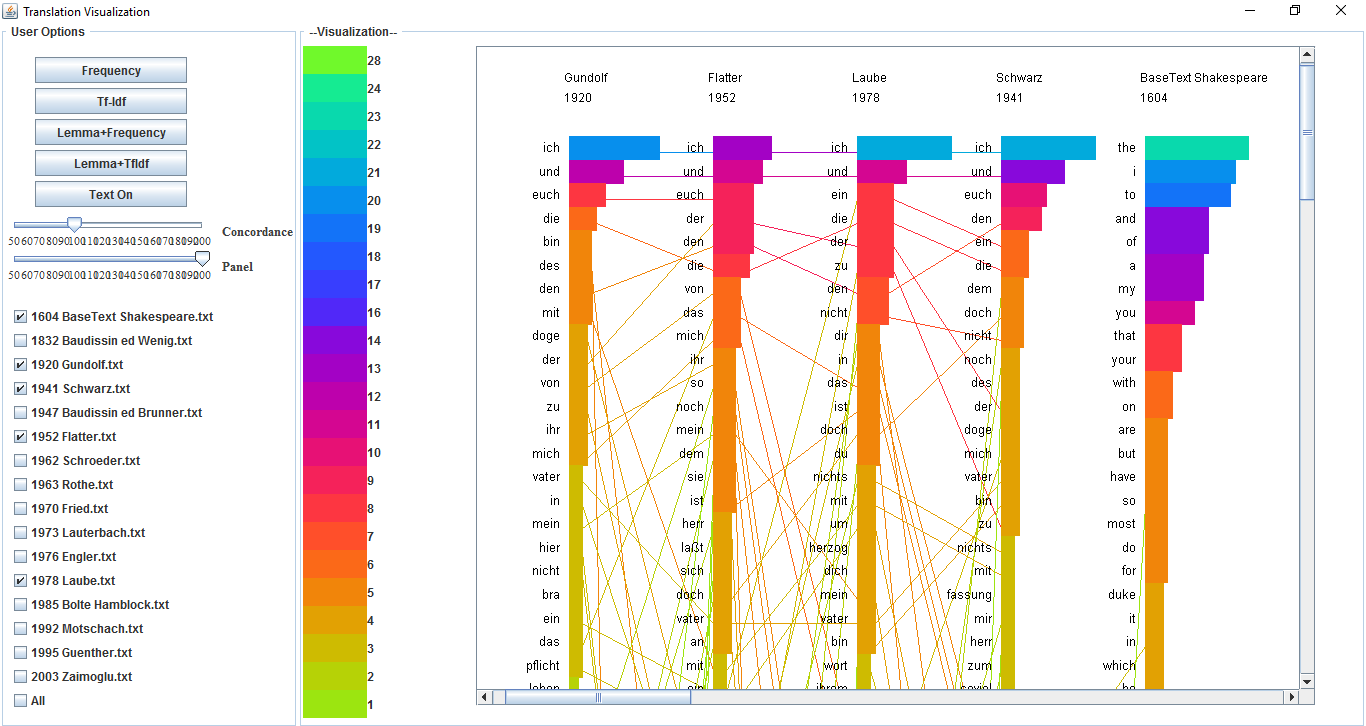
\includegraphics[width=\textwidth]{Figs/Version-Selecting-Demo}\\[1ex]
	\caption{The screenshot of version selection feature.}
	\label{fig:versionChoosDemo}
\end{figure} 

\subsection{Interaction and Selection of Terms}

On the grounds that each concordance contains a large number of terms, the ability to highlight terms defined by the user is desired. Therefore a clear view of highlighting terms comes out. 

This features are achieved by put into effect the following phases:
\begin{itemize}
	\item \textbf{} Obtain the mouse pointer’s co-ordinates via the getPoint() in MouseEvent class.
	\item \textbf{} Calculate which item region the point lies in. In this process, the regions of the display are divided as term regions. As the value of each region is calculated during data reading phase, the point passed from mouseClicked() method can be used to identify which region the point belongs. Further more, the Item object of this block is singled out and rendered. 
	\item \textbf{} Identify the Item objects in other concordances sharing the same term, and pass them to [the highlighting method].
	\item \textbf{} Highlight the blocks of all selected Item objects. In this step, lines are drawn around the rectangles. 
	\item \textbf{} Make other blocks transparent by setting the transparency values. 
	\item \textbf{} Overwrite the colour values of all lines to make the lines connecting two highlighted items are also highlighted, while other lines becoming semitransparent.
	\item \textbf{} Retrieve the translation of this term and highlight the blocks in the original English version.	
\end{itemize}

As a result, by clicking one single rectangle in the panel, the rectangle is highlighted and given an border while the colour of the other rectangles become transparent.additionally, the lines connecting identical terms are likewise highlighted by setting other lines transparent. An illustration of this feature can be seen in Figure \ref{fig:highlightView}

\begin{figure}[H]
	\centering	
	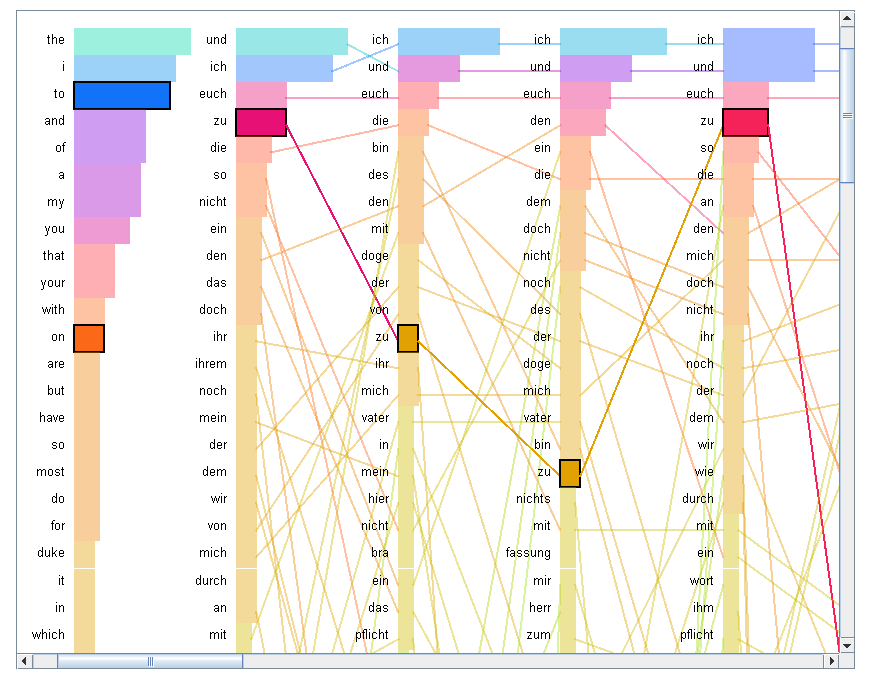
\includegraphics[scale=0.6]{Figs/Highlight-Terms}\\[1ex]
	\caption{A visualisation of highlighting certain word in the concordance.}
	\label{fig:highlightView}
\end{figure} 

\subsection{Colour Mapping}

The colours selected are related by the number of occurrences of terms in each concordance. To increase visibility, the visualization should use as large a range of colours possible., which can be achieved through colour mapping. In this project, we instantiate the ColorLegendPanel class to fulfill this role. In addition, values of the frequency are displayed in the Colour Mapping view. The following is the process took to implement this function: 
\begin{itemize}
	\item \textbf{} Retrieve the colour value of each item from the DataReader class. An explanation of colour values can be found in Data Reading chapter.
	\item \textbf{} Instantiate JLabel objects as representation for colours.
	\item \textbf{} Add the JLabel objects to the panel.
	\item \textbf{} Display frequency values beside colour blocks.
\end{itemize}

The demo of Colour Mapping is shown in Figure \ref{fig:colourMapping}.
\begin{figure}[H]
	\centering	
	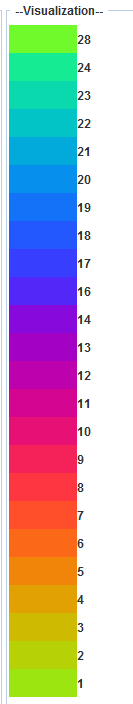
\includegraphics[scale=0.5]{Figs/Color-Mapping}\\[1ex]
	\caption{A screenshot of colour mapping.}
	\label{fig:colourMapping}
\end{figure} 

\subsection{Interactive Colour Legend}

Colour mapping is not reserved for just static visualizations, we can dynamically change the map to create an interactive visualization. In this project, we add a feature enabling users to interact with the colour legend. If the user clicks a label in the colour legend, all blocks of that colour in the concordance view will be highlighted. This function is performed by identifying all items possessing the same frequency value. As illustrated in the Design chapter, an index of frequency values is generated in the DataReader class. After data reading phase, we can access this list of frequency values through an accessor method. By iterating through all values in the list, the ConcordancePanel class, where the list of Version objects is overwritten and the panel is repainted.

As a result, by clicking one colour block in colour legend, all items sharing the same frequency, or colour, are highlighted using the same methods of highlighting described in Interaction and Selection of Terms chapter. Figure \ref{fig:interactiveColourMapping} serves as a demo to illustrate this feature.
\begin{figure}[H]
	\centering	
	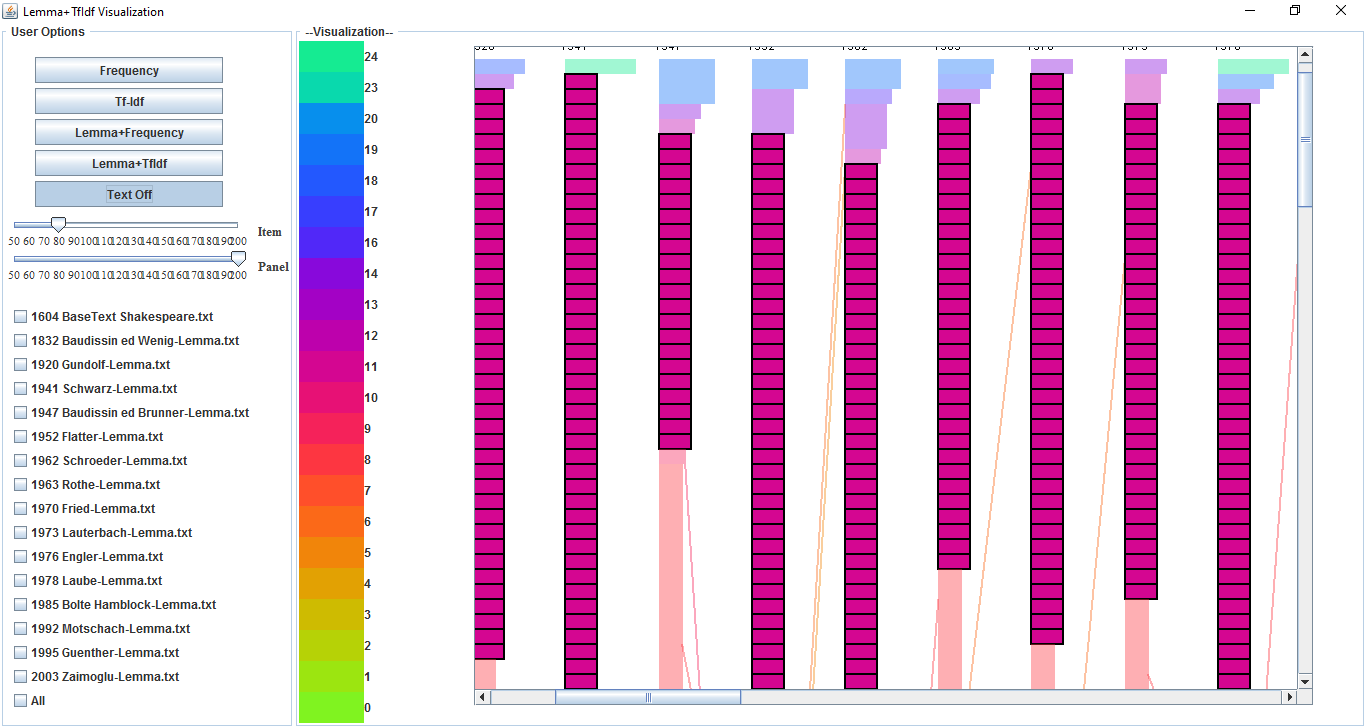
\includegraphics[width=\textwidth]{Figs/Colour-Legend-Interation}\\[1ex]
	\caption{A screenshot of highlighting items sharing the same number of frequency.}
	\label{fig:interactiveColourMapping}
\end{figure} 

\subsection{Lemmatisation}

The lemma visualisation is a significant feature in this project. Lemma is a linguistic term which is described as the dictionary form of a word. Word 'decide' is the lemma for 'decided', 'decides'and 'deciding'. Accordingly, lemmatisation is the process to obtain the lemma for each word. To achieve the effect of lemma view, several steps are necessary:
\begin{itemize}
	\item \textbf{} Obtain the German lemma corpus which contains an index of lemmas and words.
	\item \textbf{} Compare the words in our German translation corpus with the words in the German lemma corpus, and find the lemma for each term in our corpus.
	\item \textbf{} Store all the lemmas  found and generate a new lemma index.
	\item \textbf{} Apply the lemmatisation results into visualisation.
\end{itemize}
For this project, an inevitable dilemma is the limited resources of German lemma corpus. As illustrated in Data Characteristics chapter, no relevant German lemma corpus was provided when we start this project. Also, German, as an affected language, is difficult to lemmatise. During this process, we attempted two solutions: Treetagger and DeReWo, which we explained in following sections.

\subsubsection{TreeTagger}

As introduced in the Technology Choices chapter, TreeTagger is a tool for annotating text data and lemma information. Figure \ref{fig:treeTaggerUI} shows the User Interface of the TreeTagger. While applying this tool in the lemmatising task of the project, we found this tool has the following advantages:

\begin{figure}[H]
	\centering	
	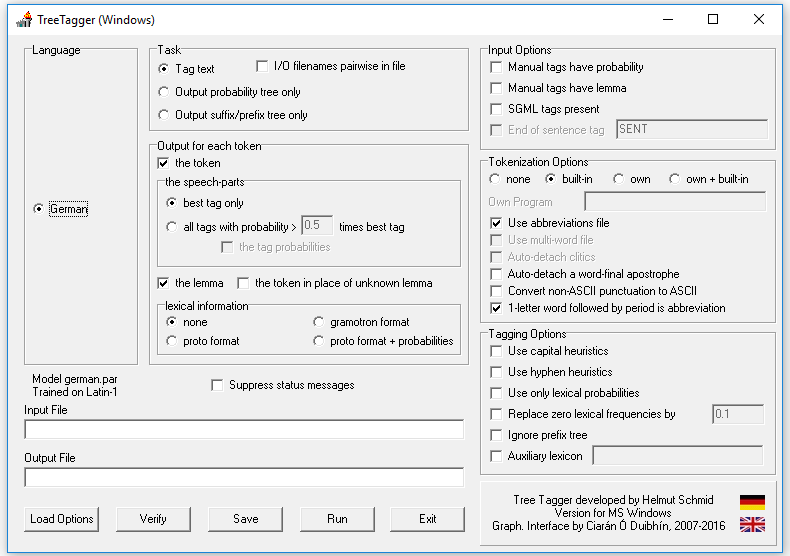
\includegraphics[scale=0.6]{Figs/TreeTaggerInterface}\\[1ex]
	\caption{The User Interface of the TreeTagger.}
	\label{fig:treeTaggerUI}
\end{figure} 

\begin{itemize}
	\item \textbf{} The software is easy to obtain, without any redundant procedures such as registration. The tool can be downloaded directly from the website \url{http://www.cis.uni-muenchen.de/~schmid/tools/TreeTagger/}.
	\item \textbf{} The user interface of the tool is clear and easy to use.
	\item \textbf{} The software takes as parameters a .txt file and returns a .txt file of results.	
\end{itemize}

However, there are also some problems we encountered:
\begin{itemize}
	\item \textbf{} The format of the text file must be encoded in Latin-1, while the text file we have is encoded in UTF-8. Therefore, some German terms with special characters cannot be recognised by the tool.
	\item \textbf{} From the results we achieved, the tool cannot recognise words with capital letters. 
	\item \textbf{} The tool cannot be used to lemmatise a batch of files at one time, which is not appropriate for a project which needs to process large datasets. 	
\end{itemize}

We connected a domain expert, Dr. Tom Cheesman from the College of Arts and Humanities at Swansea University, to evaluate the results of the lemmatisation produced by TreeTagger. Due to the low accuracy of the results for the data in this project, this solution was discarded in the end.

\subsubsection{DeReWo}

DeReWo is a project done by 'The Institute for the German Language'. This project aims at developing methods to create frequncy-based ranking list of lemmas based on random virtual corpora. In the DeReWo website \url{http://www1.ids-mannheim.de/direktion/kl/projekte/methoden/derewo.html?L=1}, there are some downloadable resources of German lemma, including 'DeReKo-2014-II-MainArchive-STT.100000.freq', which is a file storing top 100,000 German words, lemmas and POS. The format of this document is .freq, which can be edited in Visual Studio Code. It also can be read by Java directly. Using this corpus, we successfully obtained all the lemmas for each term in the \emph{Othello} corpus for this project.

There are several phases of using DeReWo to generate lemma visualisation:
\begin{itemize}
	\item \textbf{} Read text file from \emph{Othello} corpus.	
	\item \textbf{} Read German lemma corpus file.
	\item \textbf{} Search for the lemma of each term.
	\item \textbf{} Store the lemma in a new text file. In this step, we create 15 .txt files for all German translations. For each version of \emph{Othello} translation, the two files (\emph{Othello} source file and lemma file) are served as an index for words and lemmas.
	\item \textbf{} Replace all terms with their lemmas and visualise the new results.
\end{itemize}	

Figure \ref{fig:lemmaView} shows the outcome of the lemma visualisation. 

\begin{figure}[H]
	\centering	
	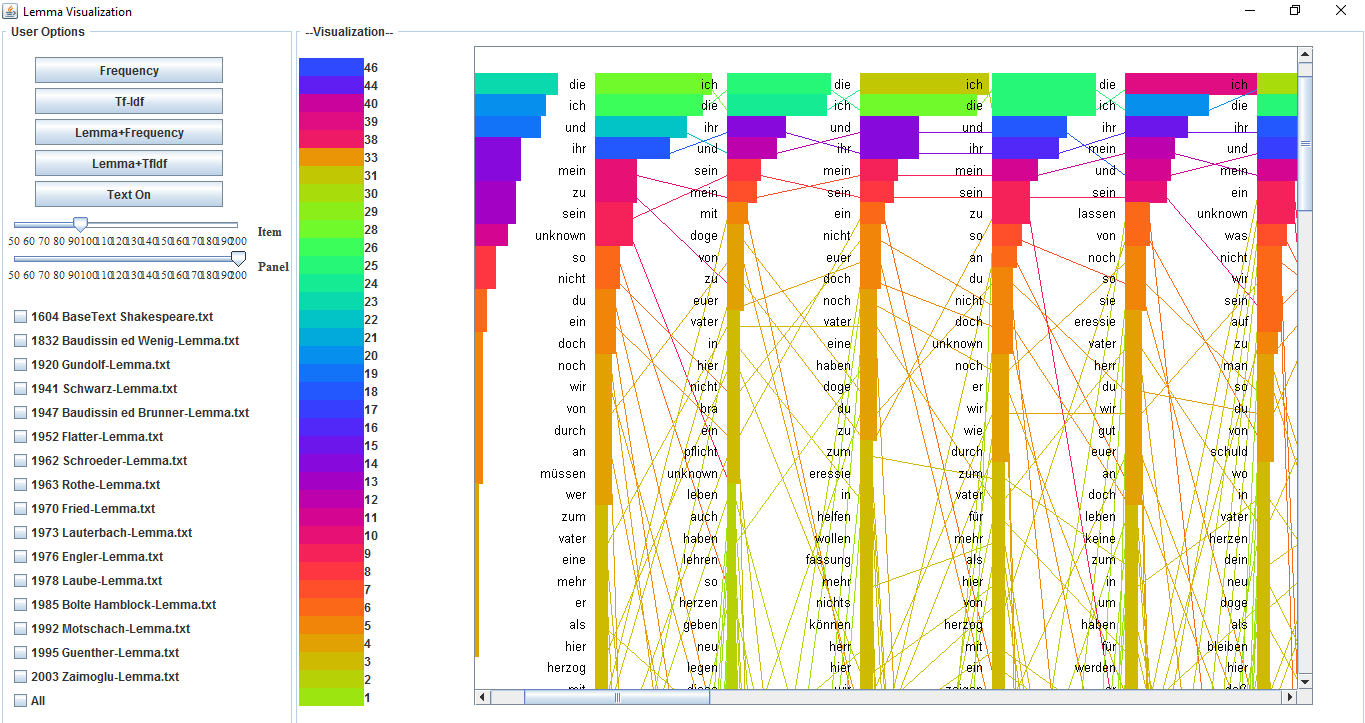
\includegraphics[width=\textwidth]{Figs/LemmaView}\\[1ex]
	\caption{A screenshot of Lemma view.}
	\label{fig:lemmaView}
\end{figure} 

\subsection{Tf-Idf}

Tf-Idf visualisation is an important feature in this project. As explained in the Design chapter, the Tf-Idf value represents the weightings of words, which also means we can get rid of unimportant words, namely stopping words. Therefore, the visualisation provided will be more helpful for researchers to study the varieties of translation. To fulfill this function, the most challenging step is to implement the formula of the Tf-Idf into code \cite{Manning2009}. The TfIdfCalculator class is created to process the Tf-Idf values.

The Tf-Idf visualisation generation process goes through the following steps:

\begin{itemize}
\item \textbf{} Calculate term frequency value. This step is done in the data reading stage. The Tf value hence can be achieved from DataReader object.
\item \textbf{} Calculate Idf value.  
\item \textbf{} Replace the frequency with Tf-Idf value.
\item \textbf{} Visualise according to the new results.
\end{itemize} 

There are two visualisations generated using Tf-Idf value: 

\begin{itemize}
	\item \textbf{} a visualisation use the Tf-Idf value of the word without lemmatising. The result is shown in Figure \ref{fig:tfIdfView};
	\item \textbf{} a visualisation use the Tf-Idf value for the lemma of the word. The result is displayed in Figure \ref{fig:tfIdfLemma}.
\end{itemize}

\begin{figure}[H]
	\centering	
	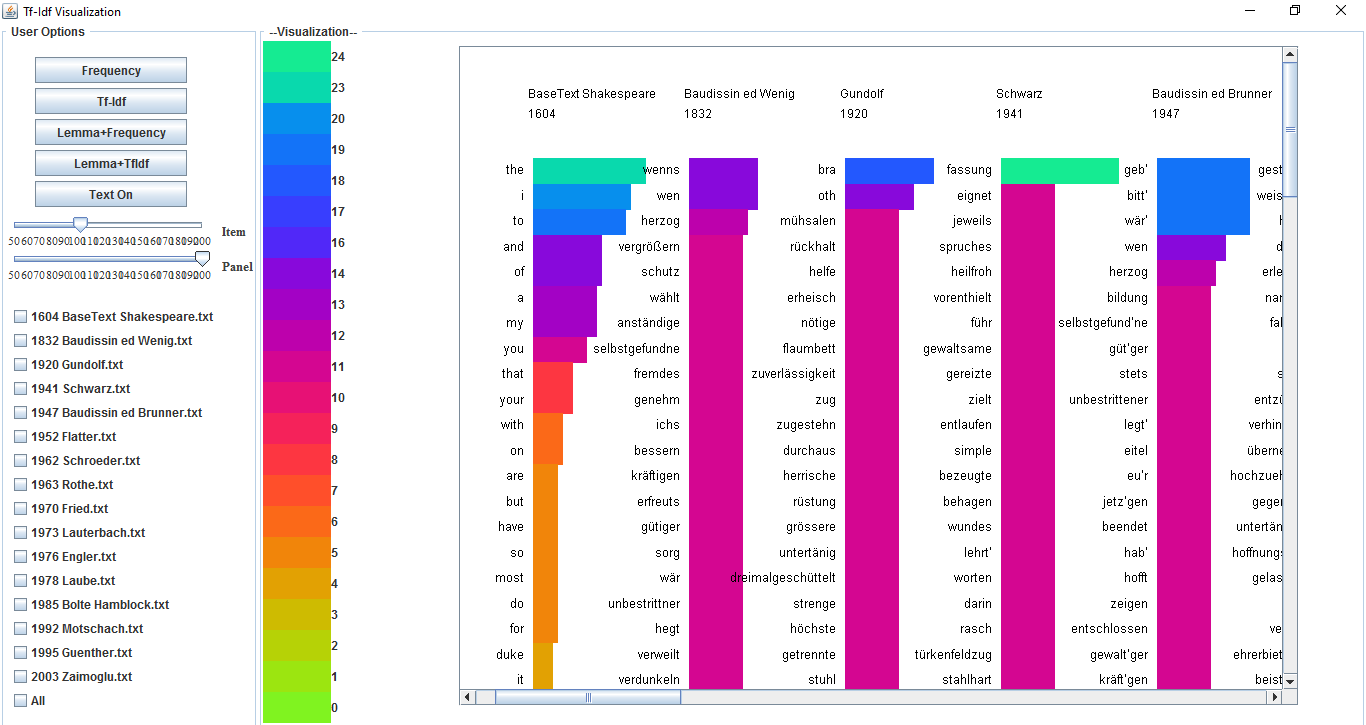
\includegraphics[width=\textwidth]{Figs/Tf-Idf}\\[1ex]
	\caption{A result of Tf-Idf visualisation.}
	\label{fig:tfIdfView}
\end{figure} 
\begin{figure}[H]
	\centering	
	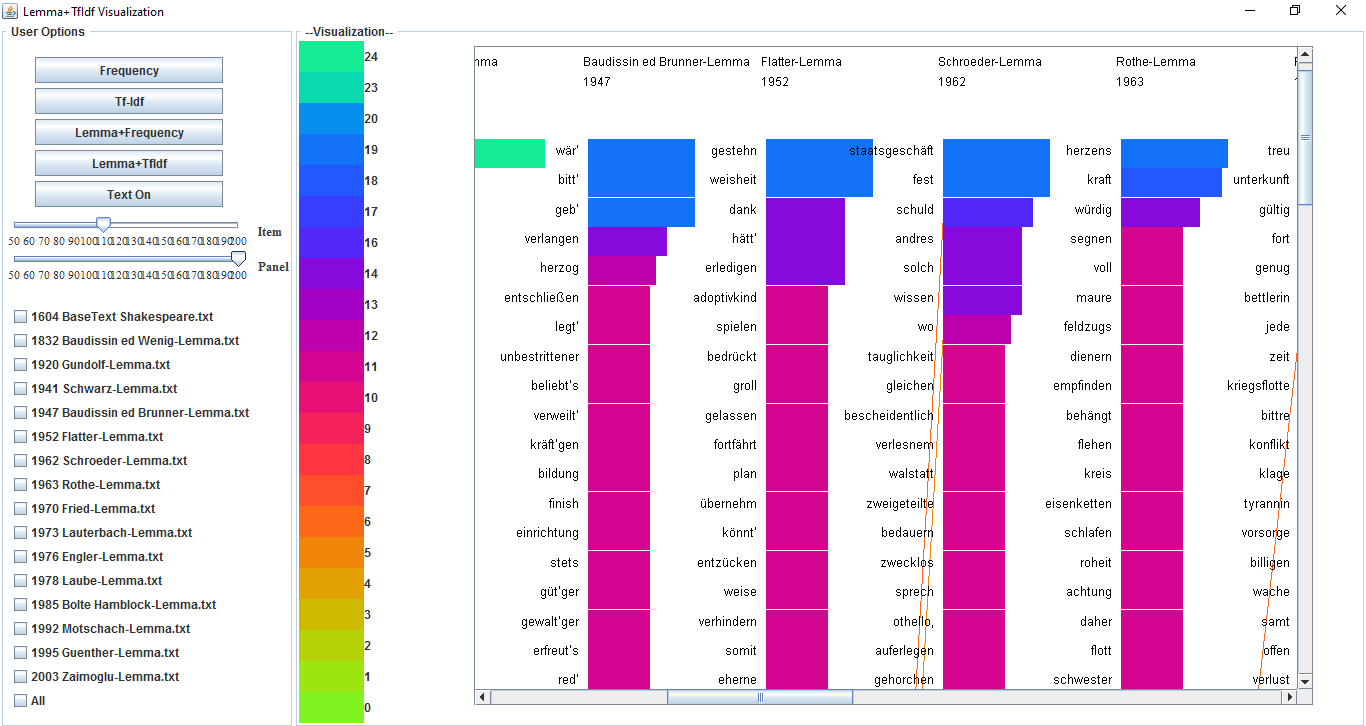
\includegraphics[width=\textwidth]{Figs/Lemma-TfIdf}\\[1ex]
	\caption{Lemma and Tf-Idf Visualisation.}
	\label{fig:tfIdfLemma}
\end{figure} 


